\documentclass{BeamerTemplate}

\title{Module 3 - Loi normale et théorème central limite}

\date{\today}

\begin{document}
\begin{frame}[t]
  \titlepage
\end{frame}

%-------------------------------------------------------------------------------------------------------------------------------------





%%%%%%%%%%%%%%%%%%%%%%%%%%%%%%%%%%%
%%%%%%%%%%%%%%%%%%%%%%%%%%%%%%%%%%%
%%%%%%%%%%%%%%%%%%%%%%%%%%%%%%%%%%%


\section{Description de la loi normale}

\begin{frame}[t]{Loi importante}

La loi normale est  la loi de probabilité la plus utilisée dans les
applications de la statistique: %Quelques raisons de sa popularité:

\begin{itemize}
\item elle modélise bien la distribution de plusieurs variables;% d'intérêt.
\item elle approxime la loi de  variables représentant une somme ou une moyenne de plusieurs mesures (théorème central limite);
\item elle mène à des résultats analytiques dans plusieurs problèmes d'inférence statistique
\end{itemize}
\end{frame}

\subsection{Propriétés}

\begin{frame}[t]{Densité de la loi normale}
On dit que $X$ suit une loi normale d'espérance $\mu$ et de variance $\sigma^2$, dénoté
\alert{$X\sim \mathcal{N}(\mu,\sigma^2)$}, lorsque sa densité est donnée par
$$f(x)=\frac{1}{\sqrt{2\pi\sigma^2}}
e^{-\frac{1}{2}\left(\frac{x-\mu}{\sigma}\right)^2},\ \ \quad
-\infty<x<\infty.$$

\begin{center}
    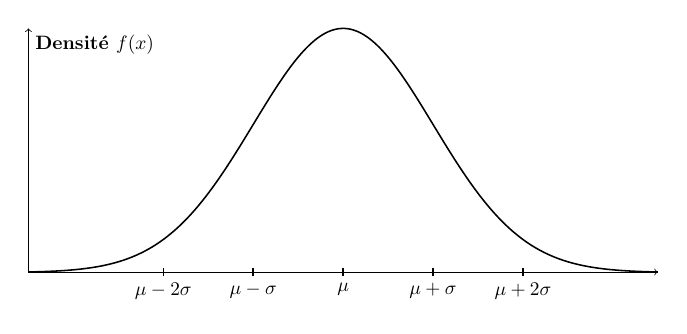
\begin{tikzpicture}[scale = 0.7]
\begin{axis}[
    no markers,
    domain=0:7,
    samples=200,
    axis lines=middle,
    ylabel={\textbf{Densité $f(x)$}},
    xtick={1.5,2.5,3.5,4.5,5.5},
    xticklabels={$ \mu-2\sigma $, $ \mu-\sigma $, $ \mu $, $ \mu+\sigma $, $ \mu+2\sigma $},
    ytick=\empty,
    enlargelimits=false,
    clip=false,
    width=13cm,
    height=6cm,
    axis line style={->},
    tick style={black, thick},
    label style={font=\bfseries}
]
\addplot[black, thick] {1/sqrt(2*pi)*exp(-(x-3.5)^2/2)};
\end{axis}
\end{tikzpicture}
\end{center}

\end{frame}

\begin{frame}[t]{Propriétés les plus importantes de la densité}
\begin{itemize}\itemsep 5mm
\item $f(x)\ge0$ pour tout $x\in\mathbb{R}$ et $\int_{-\infty}^\infty f(x)\;dx=1$
\item $\lim\limits_{x\to -\infty}f(x)=0$ et $\lim\limits_{x\to\infty}f(x)=0$
\item $f(\mu-x)=f(\mu+x)$ pour tout $x\in\mathbb{R}$  \alert{(symétrique autour de $\mu$)}
\item $f(x)$ atteint son unique maximum en $x=\mu$
\item $f(x)$ a deux points d'inflexion:  en \alert{$\mu-\sigma$} et  en \alert{$\mu+\sigma$}

\end{itemize}
\end{frame}
\begin{comment}

png("densite.png",height=5,width=8,units="in",res=90)
y<-c(-600:600)
x<-y/100
plot(x,dnorm(x,0,2), type="l",main="",
     #main=expressio\mathcal{N}(paste("Densité normale(",mu,",",sigma^2,")")),
     ylab="Densité f(x)",ylim=c(0,0.21),col=1,lwd=2,bty="l",yaxs="i",col.axis="white",cex.lab=1.5)
mtext(expressio\mathcal{N}(mu),side=1,at=0,line=1,cex=1.5)
mtext(expressio\mathcal{N}(mu+sigma),side=1,at=2,line=1,cex=1.5)
mtext(expressio\mathcal{N}(mu-sigma),side=1,at=-2,line=1,cex=1.5)
mtext(expressio\mathcal{N}(mu+2*sigma),side=1,at=4,line=1,cex=1.5)
mtext(expressio\mathcal{N}(mu-2*sigma),side=1,at=-4,line=1,cex=1.5)
dev.off()

x<-seq(-6,10,length=1000)
png("Normale-mu.png",height=5,width=6,units="in",res=130)
plot(x,dnorm(x,-1,2), type="l", main=expressio\mathcal{N}(paste("Normale(",mu,",4)")),ylab="Densité",ylim=c(0,0.4),
     col=1,lwd=2,bty="l",yaxs="i",las=1)
segments(-1,0,-1,dnorm(-1,-1,2),lty=2,col=1)
par(new=TRUE)
plot(x,dnorm(x,0,2), type="l",ylab=" ",ylim=c(0,0.4),col=2,lwd=2,bty="l",yaxs="i",las=1)
segments(0,0,0,dnorm(0,0,2),lty=2,col=2)
par(new=TRUE)
plot(x,dnorm(x,4,2), type="l",ylab=" ",ylim=c(0,0.4),col=3,lwd=2,bty="l",yaxs="i",las=1)
segments(4,0,4,dnorm(4,4,2),lty=2,col=3)
text<-c(expressio\mathcal{N}(paste(mu,"= -1 ")),expressio\mathcal{N}(paste(mu,"=  0 ")),expressio\mathcal{N}(paste(mu,"=  4 ")))
legend(-5.5,0.4,legend=text,col=1:3,lty=1,lwd=2)
dev.off()

png("Normale-sigma.png",height=5,width=6,units="in",res=130)
plot(x,dnorm(x,4,1), type="l", main=expressio\mathcal{N}(paste("Normale(4,",sigma^2, " )")),ylab="Densité",ylim=c(0,0.4),
     col=1,lwd=2,bty="l",yaxs="i",las=1)
segments(4,0,4,dnorm(4,4,1),lty=2,col=1)
par(new=TRUE)
plot(x,dnorm(x,4,2), type="l",ylab=" ",ylim=c(0,0.4),col=2,lwd=2,bty="l",yaxs="i",las=1)
segments(4,0,4,dnorm(4,4,2),lty=2,col=2)
par(new=TRUE)
plot(x,dnorm(x,4,3), type="l",ylab=" ",ylim=c(0,0.4),col=3,lwd=2,bty="l",yaxs="i",las=1)
segments(4,0,4,dnorm(4,4,3),lty=2,col=3)
text<-c(expressio\mathcal{N}(paste(sigma^2," = 1 ")),expressio\mathcal{N}(paste(sigma^2," = 4 ")),expressio\mathcal{N}(paste(sigma^2," = 9 ")))
legend(-5.5,0.4,text,col=1:3,lty=1,lwd=2)
dev.off()
\end{comment}

\begin{frame}[t]{Les deux paramètres de la loi $\mathcal{N}(\mu,\sigma^2)$}
Pour calculer des probabilités à partir de ce modèle, il faut donner des valeurs à deux paramètres:% $\mu$ et $\sigma^2$.

\begin{itemize}
\item{\bf Espérance:}  $E(X)=\mu$.  %$E(X-\mu)=\int_{-\infty}^\infty (x-\mu)\frac{1}{\sqrt{2\pi\sigma^2}} e^{-\frac{1}{2}\left(\frac{x-\mu}{\sigma}\right)^2}dx$. En posant $u=\{(x-\mu)/\sigma\}^2/2$, on trouve que $E(X-\mu)=0$, donc que $E(X)=\mu$ (voir détails dans le livre).
\item{\bf Variance:}  $V(X)=E[(X-\mu)^2]=\sigma^2$.
\end{itemize}
\begin{center}
    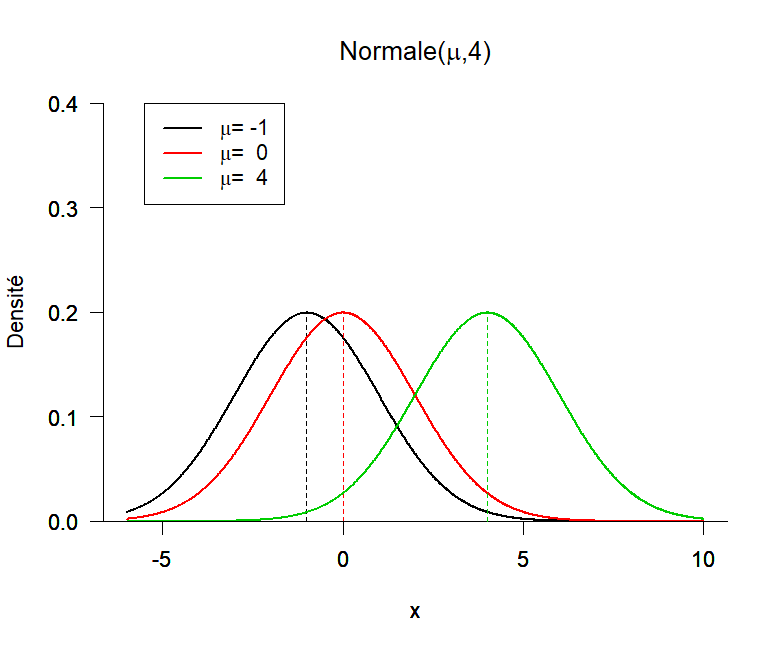
\includegraphics[width=6cm]{Images/Module 3/Normale-mu.png}
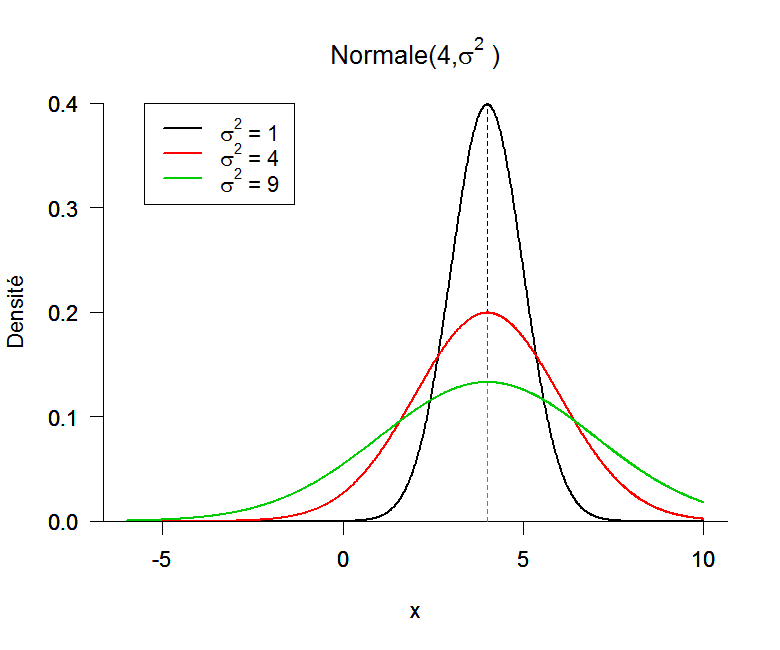
\includegraphics[width=6cm]{Images/Module 3/Normale-sigma.png}
\end{center}


\end{frame}


\begin{frame}[plain, t]%{Questions}

\centerline{\LARGE\bf \alert{QUIZ !}}
\bigskip
La longueur $X$ des lattes de bois coupées par une machine est distribuée selon une loi normale de paramètres $\mu=2400$ mm et $\sigma^2=4$ mm$^2$.  Laquelle des deux probabilités est la plus grande?
\bigskip

\begin{enumerate}
  \item $P(X<2396)$ ou $P(X>2404)$ ?
    \vspace{2cm}
  \item $P(2396<X<2397)$ ou $P(2401<X<2402)$ ?
    \vspace{2cm}
\end{enumerate}

\end{frame}
\subsection{Standardisation}

\begin{frame}[t]{Loi normale centrée-réduite}
\small
\begin{itemize}\itemsep5mm
\item {\bf Loi normale standard (ou loi normale centrée-réduite):}\\ Lorsque $\mu=0$ et $\sigma^2=1$:  \alert{$Z\sim \mathcal{N}(0,1)$}
%Soit $\phi(x)=(2\pi)^{-1/2}e^{-x^2/2}$, la densité de la loi $\mathcal{N}(0,1)$, appelée \alert{loi normale standard}. La fonction de répartition de la $\mathcal{N}(0,1)$ est
\item {\bf Fonction de répartition de la $\mathcal{N}(0,1)$:}
$$F(z)={\color{red}{\Phi(z)}}=P(Z\leq z)%=\int_{-\infty}^x \phi(u)\;du
=\int_{-\infty}^z\frac{1}{\sqrt{2\pi}}\;e^{-\frac{1}{2}u^2}du,\quad\ -\infty<z<\infty.$$
Il n'y a pas de solution analytique à cette intégrale.

\item{\bf Table des valeurs de $\Phi(z)$:}  \\
Disponible dans les livres de probabilités et de statistique, et dans des logiciels tels Excel, Matlab, Maple, R, etc.
\item Toutes les variables aléatoires suivant une loi normale $\mathcal{N}(\mu,\sigma^2)$ peuvent se transformer en normales centrées-réduites par standardisation.  \\

\end{itemize}
\end{frame}

\begin{frame}[t]{Standardisation de $\mathcal{N}(\mu, \sigma^2)$ en $\mathcal{N}(0,1)$}
\begin{itemize}
\item {\bf Standardisation:} Pour utiliser la table de $\Phi(z)$, on doit transformer la variable $X$ qui suit une $\mathcal{N}(\mu,\sigma^2)$:

\bigskip
    \begin{enumerate}
    \item Il faut  "centrer" $X$, i.e. ramener sa moyenne à 0:
    $$X\sim \mathcal{N}(\mu,\sigma^2)\quad\Rightarrow\quad X-\mu\sim \mathcal{N}(0,\sigma^2)$$
    \item Il faut "réduire" $X-\mu$, i.e. amener l'écart-type à 1:
    $$X-\mu\sim \mathcal{N}(0,\sigma^2)\quad\Rightarrow\quad \frac{X-\mu}{\sigma}\sim \mathcal{N}(0,1)$$
    \end{enumerate}
\end{itemize}
  \end{frame}

\begin{frame}[t]{Standardisation: justification mathématique}

  \begin{itemize}

\item<1->  Soit $X\sim \mathcal{N}(\mu,\sigma^2)$. On a que
{\small
\begin{align*}
F(x)= P(X\le x)&=\int_{-\infty}^x \frac{1}{\sqrt{2\pi\sigma^2}}
e^{-\frac{1}{2}\left(\frac{t-\mu}{\sigma}\right)^2}\;dt\\
&=\int_{-\infty}^{(x-\mu)/\sigma}\frac{1}{\sqrt{2\pi}}e^{-\frac{1}{2}z^2}\;dz\\
&=\Phi\left(\frac{x-\mu}{\sigma}\right)\;=\;\Phi(z),\ \text{où\ }z=(x-\mu)/\sigma.
\end{align*}
}
\item<2-> En résumé: si \alert{ $X\sim \mathcal{N}(\mu,\sigma^2)$} alors \alert{$Z=\displaystyle\frac{X-\mu}{\sigma}\sim \mathcal{N}(0,1)$}.\ \
    Seule une table de la loi $\mathcal{N}(0,1)$ est requise pour calculer des probabilités impliquant la loi normale, peu importe la valeur des paramètres!
\end{itemize}
\end{frame}

\begin{frame}[t]{Standardisation}
    Petit truc qui sera utile plus tard (module 6 et suite):
\begin{itemize}\itemsep 8mm
    \item On sait que si $X\sim\mathcal{N}(\mu, \sigma^2)$, $E(X)=\mu$ et $V(X)=\sigma^2$;
    \item On peut donc réécrire $X\sim\mathcal{N}(E(X), V(X))$;
    \item La standardisation est donc $\displaystyle Z = \frac{X-E(X)}{\sqrt{V(X)}}$.
\end{itemize}
    
\end{frame}
\begin{frame}[t]{Fonction de répartition de la loi $\mathcal{N}(0,1)$}

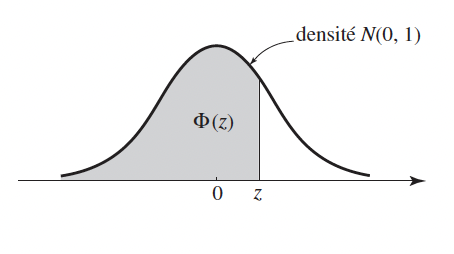
\includegraphics[scale = 0.3]{Images/Module 3/aire_proba.png}    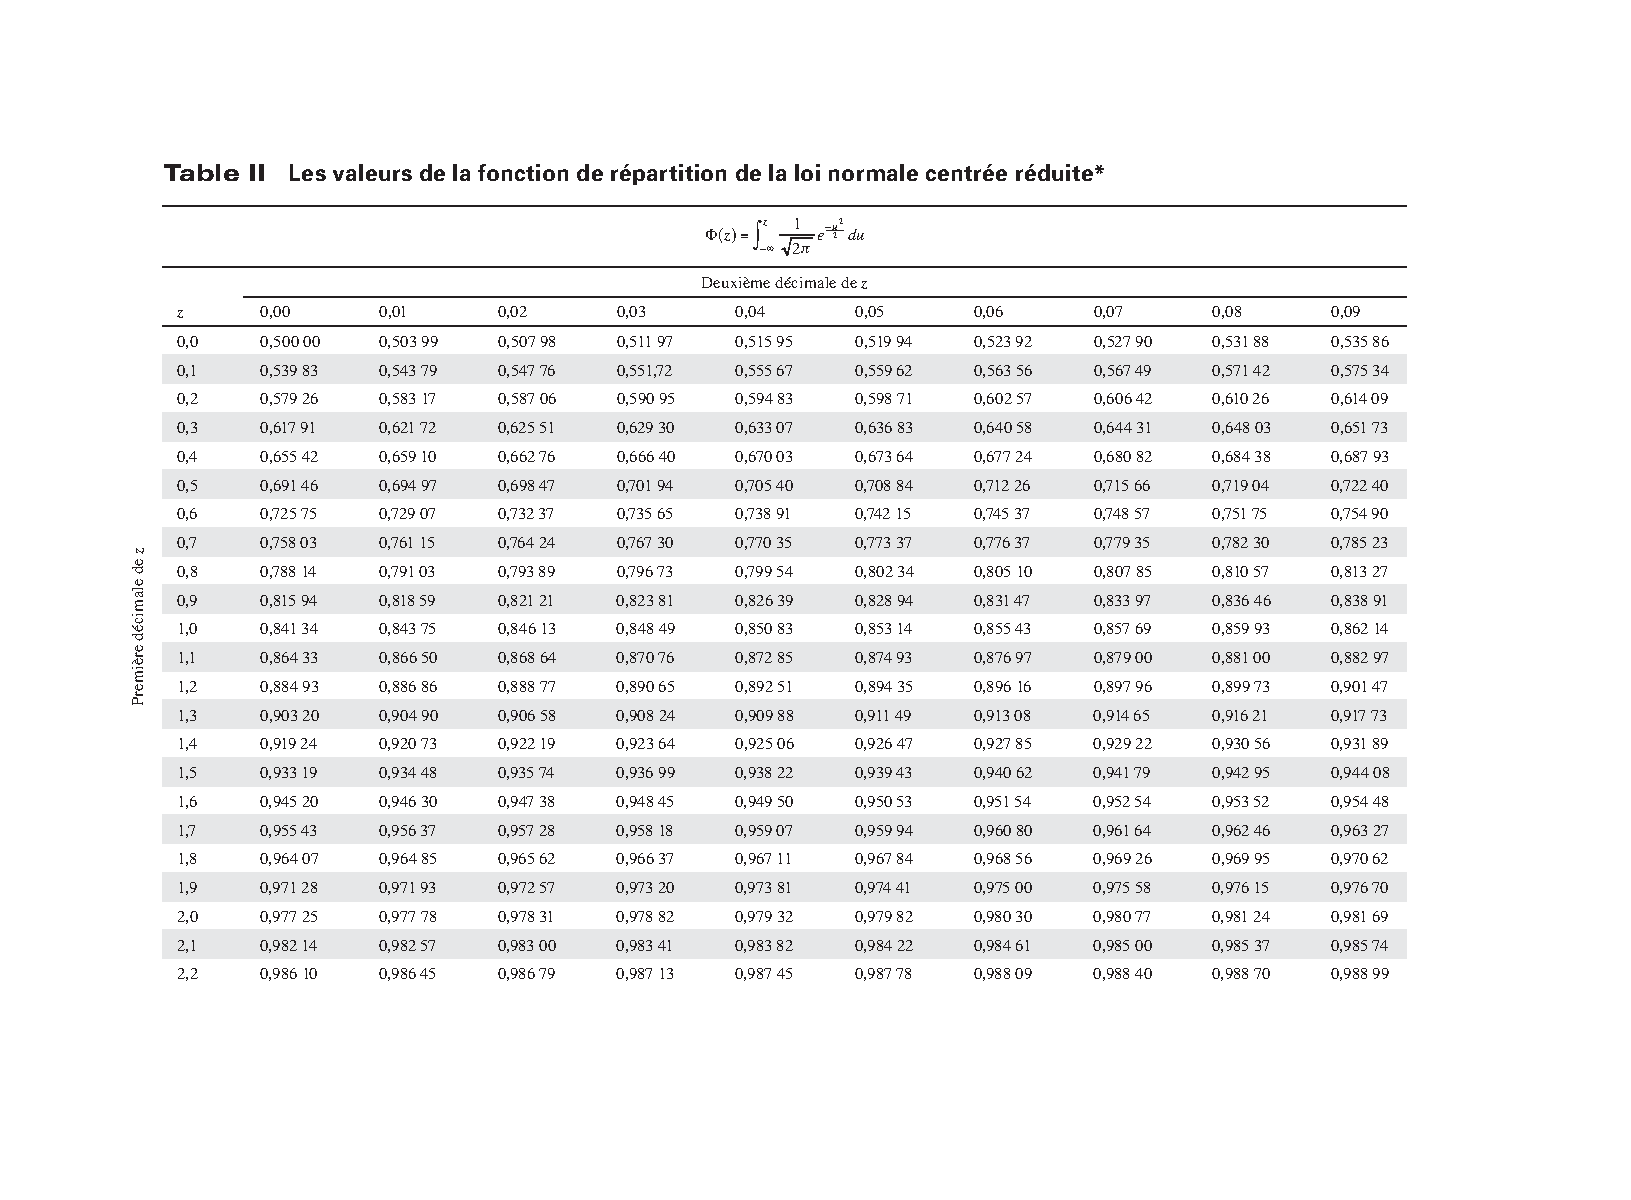
\includegraphics[scale = 0.45]{Images/Module 3/Normale_repart.pdf}



\end{frame}



\begin{frame}[t]{Exemple 1}

{\small
Environnement Canada mesure la vitesse du vent (en km/h) à chaque heure à la station météo de l'aéroport Jean-Lesage. Supposons que la vitesse horaire en janvier peut être vue comme une v.a. normale de moyenne 17 et d'écart-type 8.
}



\end{frame}

\begin{frame}[t]{Exemple 1 (suite)}

{\small
\begin{enumerate}[(i)]
\item Quelle est la probabilité qu'une mesure de la vitesse horaire dépasse  27 km/h?

\end{enumerate}}

\end{frame}

\begin{frame}[t]{Exemple 1 (suite)}

{\small
\begin{enumerate}[(ii)]
\item Quelle proportion des mesures sont comprises entre 5 et 25 km/h?
% 0.77453

\end{enumerate}}

\end{frame}

\begin{frame}[t]{Exemple 1 (suite)}

{\small
\begin{enumerate}
\item[(iii)] Quelle est la vitesse, disons $v_1$, telle que 97,5\% des mesures horaires représentent une vitesse inférieure à $v_1$? % 32.68 km/h
\end{enumerate}}

\end{frame}



\begin{frame}[plain, t]%{Questions}


\centerline{\LARGE\bf \alert{QUIZ !}}
\bigskip

\small
Quelle est la vitesse $v_2$ telle que 80\% des mesures horaires sont supérieures à $v_2$? % 10.28 km/h
\vspace{5.5cm}

\end{frame}

\section{Additivité de la loi normale}

\begin{frame}[t]{Loi d'une combinaison linéaire de v.a. normales}
Supposons que $X_1,X_2,\ldots,X_n$ sont des v.a. \alert{indépendantes}
et que $X_1\sim \mathcal{N}(\mu_1,\sigma^2_1),\; X_2\sim \mathcal{N}(\mu_2,\sigma^2_2),\; $ etc.

\begin{itemize}
\item On s'intéresse à la somme des $X_i$.
    % Soit $Y=X_1+X_2+\cdots+X_n$. Alors
    ${\color{green}{X_1+X_2+\cdots+X_n}}\sim \mathcal{N}({\color{blue}{\mu_1+\cdots+\mu_n}},{\color{purple}{\sigma^2_1+\cdots+\sigma^2_n}})$
    % o\`u $\mu=\mu_1+\cdots+\mu_n$ et $\sigma^2=\sigma^2_1+\cdots+\sigma^2_n$.
\item On s'intéresse à une combinaison linéaire des $X_i$.
    %Soit $W=a_1X_1+\cdots+a_nX_n$, o\`u $a_1,\ldots,a_n$ sont des constantes. Alors
    ${\color{green}{a_1X_1+\cdots+a_nX_n}}\sim \mathcal{N}({\color{blue}{a_1\mu_1+\cdots+a_n\mu_n}},{\color{purple}{a^2_1\sigma^2_1+\cdots+a^2_n\sigma^2_n}})$
    %avec $\tilde\mu=a_1\mu_1+\cdots+a_n\mu_n$ et $\tilde\sigma^2 =a^2_1\sigma^2_1+\cdots+a^2_n\sigma^2_n$.
\end{itemize}


Si les $X_i$ ne sont pas des v.a. indépendantes, leurs combinaisons linéaires suivent quand même des lois normales et avec les moyennes données ci-dessus, mais les \alert{formules de variances doivent être ajustées afin de tenir compte des covariances (mesures de dépendance)}.

\end{frame}

\begin{frame}[t]{Exemple 2}
Le portefeuille d'actions de votre firme est constitué à
\begin{itemize}
\item 20\% d'actions de ABC (rendement moyen 0,12)
\item 30\% d'actions de EFG (rendement moyen 0,15)
\item 50\% d'actions de WXY (rendement moyen 0,15)
\end{itemize}

On vous dit que les rendements des trois titres sont des v.a.
normales indépendantes de variance 0,09. \\

Quelle est la probabilité que le rendement global de ce portefeuille excède 0,17?
%(Note: Le rendement global du portefeuille est la combinaison linéraire des rendements des actions individuelles dont les poids sont les proportions de chaque action dans le portefeuille.)

\end{frame}

\begin{frame}[t]{Exemple 2 (solution)}

{\ }
\end{frame}

\begin{frame}[t]{Exemple 3}
Le salaire des ingénieurs dans la province A suit une loi $\mathcal{N}(70,100)$, alors que dans la province B il est distribué selon une loi $\mathcal{N}(80,64)$. \\

Si on tire au hasard un ingénieur de chacune des provinces, quelle est la probabilité que le salaire de l'ingénieur de la province B excède celui de l'ingénieur de la province A?


\end{frame}

\begin{frame}[t]{Exemple 3 (solution)}

{\ }
\end{frame}

\section{Théorème central limite }

\subsection*{ }

%\begin{frame}[t]{Un résultat extrêmement utile}
%\begin{block}{Théorème 7.1}
%Soit $X_1,X_2,\ldots$ une suite de v.a. indépendantes
%avec $E(X_i)=\mu_i$ et $V(X_i)=\sigma^2_i$. Si
%$Y=X_1+X_2+\cdots+X_n$, $\bar{Y}=Y/n$ et
%$$Z_n=\frac{Y-\sum\limits_{i=1}^n\mu_i}
%{\sqrt{\sum\limits_{i=1}^n\sigma^2_i}}=
%\frac{\bar{Y}-\sum\limits_{i=1}^n\mu_i/n}
%{\sqrt{\sum\limits_{i=1}^n\sigma^2_i/n^2}},$$
%alors $Z_n\approx \mathcal{N}(0,1)$.
%\end{block}
%\alert{$\Rightarrow$\  Une somme de plusieurs v.a. indépendantes
%se comporte approximativement comme une v.a. de loi normale.}
%\end{frame}
\begin{comment}

\begin{frame}[t]{Un résultat extrêmement utile}
\begin{block}{Théorème de la limite centrale}
Soit $X_1,X_2,\ldots$ une suite de v.a. indépendantes
et identiquement distribuées avec
avec $E(X_i)=\mu$ et $V(X_i)=\sigma^2$. Si
$Y=X_1+X_2+\cdots+X_n$, $\bar{Y}=Y/n$ et
$$Z_n=\frac{Y-n\mu}
{\sigma\sqrt{n}}=
\frac{\bar{Y}-\mu}
{\sigma/\sqrt{n}},$$
alors $Z_n\approx \mathcal{N}(0,1)$.
\end{block}
\end{frame}
\end{comment}

\begin{frame}{exemple}
    \href{https://jmiron-introtcl.share.connect.posit.cloud/}{exemple introductif}
\end{frame}
\begin{frame}[t]{Un résultat très (très) utile}
\begin{Boite}{Théorème central limite}

Soit $X_1, X_2,\hdots, X_n$ des v.a. \alert{indépendantes}\\d'espérance $\mu<\infty$, \\de variance $\sigma^2<\infty$, \\ d'une même loi de probabilité (\alert{quelconque}).
\vspace{0.5cm}

Alors si $n\geq30$,
\vspace{0.5cm}

$Y\;\;=\;\;X_1+X_2+...+X_n\;\;\approx\;\; \mathcal{N}(n\mu, n\sigma^2)$

\vspace{0.5cm}

$\overline X\;\;=\;\;\displaystyle\frac{X_1+X_2+...+X_n}{n}\;\;\approx\;\; \mathcal{N}\left(\mu, \frac{\sigma^2}{n}\right)$

\end{Boite}
\end{frame}




\begin{frame}[t]{Exemple 4}

{\small
Supposons que les demandes quotidiennes en électricité de 100 usines peuvent être
vues comme des v.a. indépendantes de moyenne 10 kWh et
d'écart-type 5 kWh. \\

Quelle est la probabilité approximative que la demande quotidienne totale en électricité de ces 100 usines excède la capacité de 1100 kWh du réseau qui les alimente ?}\\

\end{frame}

\begin{frame}[t]{Exemple 4 (solution)}

{\ \ \ }
\end{frame}


\begin{frame}[t]{Réponses aux exemples}

\scriptsize
\begin{enumerate}
  \item     \begin{enumerate}[(i)]
            \item $P(X>27)=0,10565$
            \item $P(5<X<25)=0,77453$
            \item $v_1=32,68$ km/h
            %\item $10,28$ km/h
            \end{enumerate}
  \item $P(R>0,17)=0,44433$
  \item $P(X_B>X_A)=0,78230$
  \item $P(Y>1100)=0,02275$
 \end{enumerate}
\end{frame}




\end{document}